%% ---------------------------------------------------------------------------
%% Protocol-Accurate Sensor FMUs for Sensor-in-the-Loop Co-Simulation
%% of Embedded GNC Firmware
%%
%% Draft for IEEE two-column conference format (IEEEtran).
%% Target venue: SIMULTECH / SIMPAC (SCITEPRESS) -- see README for the note on
%% swapping to the SCITEPRESS class at submission time.
%%
%% Build:  pdflatex main -> bibtex main -> pdflatex main -> pdflatex main
%% ---------------------------------------------------------------------------
\documentclass[conference]{IEEEtran}

\usepackage{cite}
\usepackage{amsmath,amssymb,amsfonts}
\usepackage{graphicx}
\usepackage{booktabs}
\usepackage{array}
\usepackage{url}
\usepackage{xcolor}
\usepackage[hidelinks]{hyperref}

\graphicspath{{figures/}}

% A compact monospace helper for register names / identifiers.
\newcommand{\code}[1]{\texttt{\small #1}}

\begin{document}

\title{Protocol-Accurate Sensor FMUs for\\
       Sensor-in-the-Loop Co-Simulation of Embedded GNC Firmware}

% For a double-blind SCITEPRESS submission, replace the author block with
% \author{\IEEEauthorblockN{Anonymous Author(s)}}.
\author{\IEEEauthorblockN{Onur Tuncer}
\IEEEauthorblockA{Faculty of Aeronautics and Astronautics\\
Istanbul Technical University\\
Istanbul, Turkey\\
Email: onur.tuncer@itu.edu.tr}}

\maketitle

\begin{abstract}
Functional Mock-up Interface (FMI) co-simulation is widely used to test
guidance, navigation and control (GNC) software against a plant model, but the
sensor boundary is almost always crossed as idealized floating-point physical
quantities. This bypasses precisely the code that fails most often on real
hardware: the byte-level driver and protocol-parsing stacks that turn a
receiver's UART stream or an inertial part's SPI registers into engineering
units. We present \emph{protocol-accurate sensor FMUs}: co-simulation slaves
that take noiseless truth in over FMI, apply a grade-specific stochastic error
model, quantize to register counts, and emit \emph{wire-exact} protocol frames
on the bus the physical part actually uses---so the \emph{unmodified} target
firmware parses exactly the bytes it will see in flight, checksums included.
A sensor's FMI output set is deliberately empty; the byte stream is its output.
We show that this pattern captures behavior a value-level FMU cannot: a receiver
losing its navigation fix to export-control (COCOM) dynamics limits; a MEMS
IMU modeled as a \emph{polled} SPI peripheral with a register map, a sample
FIFO, and a sticky overflow bit; and a magnetometer whose first useful reading
does not exist until a blocking, multi-transaction SET/RESET handshake has
measured and removed a bridge offset the size of Earth's whole field. Because
each error model is the exact inverse of the on-target conversion routine, a
round-trip test pins the simulator and the flight code to each other. We
instantiate five sensors in a single embedded framework---three of them as
register-accurate parts (a MEMS IMU on SPI, a Bosch BMP390 and a MEMSIC
MMC5983MA on I$^2$C)---and validate four end-to-end against a verified 6-DoF
two-stage-rocket plant. The receiver in that run is COCOM-limited and stops
navigating $31$~s after lift-off, so the GPS statistic is the whole of what a
real receiver would have yielded: over the $312$ fixes of $2001$ epochs it
carries, the decoded-fix error RMS matches the injected noise to the centimetre
($2.12$~m horizontal against $1.5\sqrt{2}$~m expected). The inertial stream is
unaffected by that outage---$20{,}000$ of $20{,}010$ samples survive the full
noise-model$\rightarrow$encoder$\rightarrow$SPI-transport$\rightarrow$
on-target-driver chain with zero checksum errors across $48{,}021$ transfers;
$2{,}000$ barometric conversions cross $42{,}009$ I$^2$C transactions and are
recovered by running the real Bosch compensation polynomial forward against an
FMU that inverted it; and the magnetometer driver measures the simulated part's
$+16.2/{-}10.3/{+}8.5$~\textmu T bridge offset at bring-up and removes it,
without which the same samples put heading $28^\circ$ out. The same firmware
object code runs unchanged across FMI co-simulation, instruction-accurate
(Renode) simulation, and physical STM32 hardware.
\end{abstract}

\begin{IEEEkeywords}
FMI, co-simulation, software-in-the-loop, sensor emulation, embedded firmware,
GNC, hardware-in-the-loop, register-level device models, verification and
validation.
\end{IEEEkeywords}

% ===========================================================================
\section{Introduction}
% ===========================================================================
The Functional Mock-up Interface (FMI)~\cite{fmi2020,blochwitz2011fmi} has
become the lingua franca for coupling heterogeneous simulation tools, and
co-simulation is now routine in the verification of guidance, navigation and
control (GNC) software~\cite{gomes2018cosim}. A typical setup couples a plant
model---vehicle dynamics, environment, actuators---to the control software and
exchanges signals across the FMI boundary as scalar reals: position in metres,
angular rate in radians per second, magnetic field in microtesla.

That convenience hides a validation gap. On real hardware, GNC software does not
receive metres and radians. It receives a stream of bytes from a GNSS receiver's
UART, and the contents of data registers read over SPI or I$^2$C from an
inertial measurement unit (IMU). Between those bytes and the floating-point
quantities a control law consumes sits a substantial, historically bug-prone
body of code: framing and synchronization, checksum validation, little-endian
scaled-integer decoding, register-map sequencing, FIFO management, and
fixed-point-to-SI conversion with a full-scale range the driver---not the wire
format---must know. A value-level sensor FMU that emits clean reals exercises
\emph{none} of it. The software under test in the lab is therefore not the
software that flies.

Hardware-in-the-loop (HIL) rigs close this gap by driving the real buses of a
real flight computer, but they are expensive, poorly parallelizable, and
unavailable early in development. Software-in-the-loop (SIL) co-simulation is
cheap and scales to continuous integration, yet it is exactly where the
value-level shortcut is normally taken.

This paper argues that the shortcut is unnecessary. We introduce
\emph{protocol-accurate sensor FMUs}, a co-simulation pattern in which each
sensor FMU:
\begin{enumerate}
  \item takes noiseless \emph{truth} in over ordinary FMI input variables,
        driven by a physics plant through the co-simulation master's
        connections;
  \item applies a sensor-grade-specific stochastic error model and quantizes
        the result to the physical part's register counts; and
  \item emits \emph{wire-exact} protocol frames---sync bytes, scaled integers,
        checksums---on a channel that stands in for the part's real bus, with
        \emph{no FMI output variables at all}.
\end{enumerate}
The flight software decodes those frames with the \emph{unmodified} on-target
driver and conversion code. The FMI boundary carries physics; the sensor
boundary carries bytes, exactly as on the vehicle.

We make four contributions:
\begin{itemize}
  \item \textbf{The pattern} (Section~\ref{sec:method}): a reusable structure
        for byte-accurate sensor FMUs, including where unit and frame mismatches
        belong (the orchestration layer) and an \emph{inverse-model} property
        that makes the simulator and the flight code mutually self-checking.
  \item \textbf{Talker and polled transports} (Section~\ref{sec:transport}):
        modeling a GNSS receiver as a \emph{talker} that pushes frames, an
        IMU as a \emph{polled} SPI peripheral with a register map and FIFO, and
        two dissimilar I$^2$C parts whose bus conventions differ from each
        other, rather than flattening all of them to pushed byte streams.
  \item \textbf{Behavior a value-level FMU cannot express}
        (Section~\ref{sec:casestudy}): a receiver dynamics envelope (u-blox
        platform models and COCOM export limits) that revokes the fix in flight,
        FIFO-overflow semantics under a slow consumer, and a magnetometer whose
        bring-up \emph{blocks on the plant}---its bridge offset can only be
        measured by taking two real measurements in opposite magnetic
        polarities.
  \item \textbf{End-to-end validation of four sensors}
        (Section~\ref{sec:results}) against a 6-DoF two-stage-rocket plant whose
        trajectory is itself checked against published reference data, showing
        the decoded error equals the injected error to quantization, that the
        byte chain is lossless across three transports, and that the
        register-level conditioning sequence the flight code runs recovers the
        part parameter it is supposed to recover.
\end{itemize}
The pattern is realized in Hemerion, an open-source (GPLv3) C++23 embedded GNC
framework whose modules cross-compile to STM32 firmware and, unchanged, to
x86 shared libraries for co-simulation.

% ===========================================================================
\section{Related Work}
% ===========================================================================
\textbf{FMI co-simulation and signal-level SIL.} FMI~\cite{fmi2020} standardizes
model exchange and co-simulation~\cite{blochwitz2011fmi}, and Gomes et
al.~\cite{gomes2018cosim} survey the field. It is used routinely to run embedded
control software in the loop against physical
models~\cite{pedersen2016fmi,mikelsons2017virtual}. In all of this the sensor
boundary is crossed at the level of physical \emph{quantities}: the plant hands
the control code real-valued positions and rates. The same holds for the
dominant GNC simulation stacks in practice---PX4 and ArduPilot
software-in-the-loop inject idealized sensor values (e.g.\ MAVLink
\code{HIL\_SENSOR}) rather than driving the receiver's or IMU's real byte-level
parser. That driver/protocol code is exactly what our FMUs exercise.

\textbf{Frames across the FMI boundary.} The closest prior art carries
wire-level frames through FMI itself. FMI 3.0 adds an opaque \code{Binary}
variable type and clocked variables~\cite{junghanns2022fmi3}, motivated in part
by the wish to exchange whole bus frames such as CAN or SOME/IP; building on
this, the FMI Layered Standard for Network Communication
(FMI-LS-BUS)~\cite{fmilsbus2025} standardizes transporting network frames
between FMUs. We differ on three axes. \emph{(i)~Scope}: FMI-LS-BUS targets
inter-ECU \emph{network} buses (CAN/CAN-FD, with LIN/FlexRay/Ethernet in
progress), not \emph{sensor peripherals}; it has no notion of a polled
register-map/FIFO SPI device or a framed GNSS message stream, which is precisely
where sensor driver code lives. \emph{(ii)~Semantics}: it models the transport
medium with a dedicated bus-simulation FMU, whereas our contribution is the
register- and receiver-level behaviour of the part itself---fix revocation under
COCOM/platform limits, FIFO overflow under a slow poll. \emph{(iii)~Interface}:
it exchanges frames as FMI binary \emph{variables} at communication points; we
keep the byte stream off the FMI variable set entirely and emit it on the part's
real bus, so transport granularity is the bus's, not the master's step.

\textbf{Register-level sensor and virtual-platform emulation.}
Instruction-accurate emulators such as Renode~\cite{renode} run unmodified
firmware against emulated cores and model SPI/I$^2$C sensor peripherals with
register maps, and bus middleware such as Vector SIL Kit~\cite{silkit} can bridge
such virtual platforms. Register-level sensor emulation is therefore not itself
new. What is new here is bringing that fidelity \emph{to the FMI co-simulation
boundary}, co-solved with a continuous 6-DoF plant: the same sensor logic that
answers the firmware's SPI transfers is an FMU wired to the physics. Because the
sensor model is ordinary host code, one FMU can feed a native co-simulation
process or Renode's emulated UART/SPI/I$^2$C unchanged---and the same device
models are reused verbatim by the Renode-hosted software-in-the-loop tests,
rather than being a second implementation that can drift.

\textbf{Same-code SIL.} The strongest validity claim a SIL harness can make is
that it runs the identical object code that will fly. Frameworks that share a
codebase between host simulation and target firmware achieve this for control
logic; we extend it down to the sensor driver and protocol layer, normally
stubbed out in SIL precisely because value-level FMUs make it easy to.

% ===========================================================================
\section{Protocol-Accurate Sensor FMUs}
\label{sec:method}
% ===========================================================================

\subsection{Architecture}
Each sensor is packaged as an FMI 2.0 co-simulation slave with the structure of
Fig.~\ref{fig:pattern}. Truth enters as real-valued FMI \emph{inputs}, wired by
the co-simulation master from a 6-DoF plant. Inside \code{do\_step()} the FMU
applies its error model, quantizes to register counts, frames the counts into
the sensor's wire protocol, and pushes the resulting bytes onto a transport that
stands in for the physical bus. The FMU declares \textbf{no FMI outputs}: from
the master's point of view it is a pure sink, and its observable behavior is the
byte stream, exactly as a real receiver's observable behavior is its UART
traffic.

\begin{figure}[t]
\centering
\footnotesize
\setlength{\fboxsep}{4pt}
\fbox{\begin{minipage}{0.92\columnwidth}
\centering
\textsf{6-DoF plant (truth)}\\
$\big\downarrow$ \emph{FMI real inputs (Ecos connections)}\\[2pt]
\textsf{hemerion\_$\langle$sensor$\rangle$\_fmu}\\
\textsf{\scriptsize noise model $+$ quantizer $+$ packet emitter}\\
$\big\downarrow$ \emph{wire-exact frames on the part's bus}\\[2pt]
\textsf{on-target driver $+$ parser $+$ convert\_raw\_to\_si()}
\end{minipage}}
\caption{The protocol-accurate sensor FMU pattern. Physics crosses the FMI
boundary; \emph{bytes} cross the sensor boundary. The flight software is the
unmodified on-target code.}
\label{fig:pattern}
\end{figure}

This placement is deliberate. Model code lives under each sensor's \code{fmu/}
subtree and is compiled only for the host; it may use \code{<random>} and
dynamic allocation freely. The \emph{decoder}---parser and
\code{convert\_raw\_to\_si()}---lives one directory up, is MISRA-friendly
freestanding code, and is the identical translation unit the STM32 firmware
cross-compiles.

\subsection{Two fidelity tiers from one pattern}
\label{sec:tiers}
The pattern admits two tiers, and both are instantiated. A \emph{generic} model
represents a class of part---a compass-grade three-axis magnetometer, a MEMS
barometer---with a plausible register sensitivity and a talker transport; it
costs a day to write and exercises the parser and the conversion arithmetic. A
\emph{part-accurate} model transcribes one datasheet: its register map, its bus
conventions, its calibration data, and whatever internal state a driver has to
manage. Three of the five sensors here exist at the second tier (the SPI IMU,
the Bosch BMP390, the MEMSIC MMC5983MA); the generic magnetometer, barometer and
radar-altimeter emitters remain, since a scenario that only needs a field
measurement should not pay for a register file. The interesting claims in this
paper come from the second tier, and Section~\ref{sec:transport} is about what
it buys.

\subsection{The shared error model}
With the exception of the GPS receiver (which perturbs at the navigation-fix
level, since a receiver outputs a solution, not counts), every model applies the
same two-term Gaussian error per measurement channel and then quantizes:
\begin{equation}
y[k] = \operatorname{sat}\!\Big(\operatorname{round}\big(
        (x_{\text{truth}}[k] + b + w[k])\, S \big)\Big),
\label{eq:errormodel}
\end{equation}
\[
b \sim \mathcal{N}(0,\sigma_b^2), \qquad w[k] \sim \mathcal{N}(0,\sigma_w^2),
\]
where $b$ is a \emph{turn-on bias} drawn once per run per axis (the constant
offset a real part exhibits after each power-up), $w[k]$ is white measurement
noise drawn per sample, $S$ is the register sensitivity in LSB per physical
unit, and $\operatorname{sat}(\cdot)$ clips at the register's full-scale range
as silicon does rather than wrapping. Setting any $\sigma$ to zero disables that
term cleanly. Every constructor takes an RNG seed (defaulting to
\code{std::random\_device}); seed plus configuration fully determine the output
sequence, including the turn-on biases, giving bit-reproducible runs.
Table~\ref{tab:params} lists the configured error parameters for the five
models, chosen to represent the reference parts of Table~\ref{tab:sensors}.

\begin{table}[t]
\centering
\caption{Configured error-model parameters (per measurement channel). White and
turn-on-bias columns are $1\sigma$; sensitivity $S$ is shared with the on-target
\code{convert\_raw\_to\_si()} (Section~\ref{sec:inverse}). The lower block is
the part-accurate tier, whose figures are the reference part's datasheet
numbers rather than chosen ones. $^\dagger$hard iron, which conditioning does
not remove; the separately drawn bridge offset, which it does, is the row
below.}
\label{tab:params}
\footnotesize
\begin{tabular}{@{}llll@{}}
\toprule
Channel & White $1\sigma$ & Bias $1\sigma$ & Sensitivity $S$\\
\midrule
GPS horizontal & 1.5\,m/axis & --- & fix-level\\
GPS vertical   & 3.0\,m      & --- & fix-level\\
GPS speed      & 0.1\,m/s    & --- & fix-level\\
GPS course     & $1.0^\circ$ & --- & fix-level\\
IMU accel.     & 0.05\,m/s$^2$ & 0.02\,m/s$^2$ & 800\,LSB/g\\
IMU gyro       & 0.002\,rad/s & 0.001\,rad/s & 16.4\,LSB/($^\circ$/s)\\
Baro pressure  & 3\,Pa       & 50\,Pa      & 1\,LSB/Pa\\
Baro temp.     & $0.05^\circ$C & $0.5^\circ$C & 100\,LSB/$^\circ$C\\
Radar alt.\ range & 0.1\,m   & 0.05\,m     & 100\,LSB/m\\
Mag.\ (per axis) & 0.2\,\textmu T & 1.0\,\textmu T & 100\,LSB/\textmu T\\
\midrule
BMP390 pressure & 3\,Pa & 50\,Pa & 24-bit, compensated\\
BMP390 temp.    & $0.05^\circ$C & $0.5^\circ$C & 24-bit, compensated\\
MMC5983MA field & 0.04\,\textmu T & 1.0\,\textmu T$^\dagger$ & 163.84\,LSB/\textmu T\\
\quad bridge offset & --- & 16.7\,\textmu T & 18-bit unsigned\\
MMC5983MA temp. & $0.2^\circ$C & --- & 1.25\,LSB/$^\circ$C\\
\bottomrule
\end{tabular}
\end{table}

The GPS is the exception noted above: it perturbs the navigation fix directly
(a receiver reports a solution, not counts), so its noise is specified in fix
units and no register sensitivity applies.

\subsection{What a part-accurate model adds to
\texorpdfstring{\eqref{eq:errormodel}}{the shared form}}
\label{sec:partmodels}
Equation~\eqref{eq:errormodel} describes a \emph{channel}. A part has more than
a channel, and the two register-accurate I$^2$C models differ from the generic
form in opposite directions.

The BMP390's raw output means nothing on its own: the part ships 24-bit
uncompensated words that only become pascals after the floating-point
compensation polynomial of the datasheet's section~8.4~\cite{bosch_bmp390},
evaluated with
coefficients burned into each individual part's NVM at the factory. A model that
emitted counts proportional to pressure would produce a stream the real driver
would decode into the wrong number. The FMU therefore maps truth altitude
through the ICAO standard atmosphere and then \emph{numerically inverts the real
compensation polynomial}---a bisection on the monotone forward map---to find the
raw words a physical part would have converted, and serves the calibration
coefficients as the 21 NVM bytes the driver reads at bring-up. Agreement in
Section~\ref{sec:results} is therefore agreement between two executions of the
same published arithmetic across a register interface, not between a model and
its own inverse.

The MMC5983MA~\cite{memsic_mmc5983ma} needs no compensation at
all---sensitivity is a fixed $16384$~counts/gauss with no per-part NVM---and
the fidelity has to go somewhere
else, into \emph{state}. Its sensing elements are Wheatstone bridges of
anisotropic magneto-resistive film, and an on-die coil re-magnetizes them in
either direction. After a SET the applied field enters the bridges positively;
after a RESET, negatively. The bridge's own electrical offset, being electrical
and not magnetic, does not follow:
\begin{align}
\text{after SET}\quad   y_+ &= n + HS + \delta,\nonumber\\
\text{after RESET}\quad y_- &= n - HS + \delta,\label{eq:setreset}\\
\Rightarrow\quad HS &= \tfrac{1}{2}(y_+ - y_-), \quad
\delta = \tfrac{1}{2}(y_+ + y_-) - n,\nonumber
\end{align}
with $n$ the part's null-field output ($131072$ counts, mid-scale, not zero).
The measurement model therefore applies the sensing polarity to the
\emph{field} and not to $\delta$, which is what makes~\eqref{eq:setreset}
recoverable by a driver and unrecoverable by one that never runs the pair. It
also distinguishes two offsets that a value-level model would merge: $\delta$,
which SET/RESET removes, and a per-run \emph{hard-iron} vector, which is a real
field the installation adds and which no coil pulse removes. $\delta$ is drawn
each run from the datasheet's $\pm0.5$~gauss null-field tolerance taken as a
$3\sigma$ bound---i.e.\ $16.7$~\textmu T $1\sigma$, deliberately the same order
as Earth's entire field, so that a driver which skips the conditioning sequence
is wrong by roughly $100\%$ rather than by a rounding error.

\subsection{The inverse-model property}
\label{sec:inverse}
The sensitivity $S$ in~\eqref{eq:errormodel} is \emph{the same constant} the
consuming driver passes to \code{convert\_raw\_to\_si()}. Scale is configuration
both ends share---exactly as on real silicon, where the full-scale range is a
register the driver wrote, not a field on the wire. Consequently the on-target
conversion is the algebraic inverse of the FMU's quantization step: feeding the
emitted counts back through \code{convert\_raw\_to\_si()} recovers the noisy SI
sample to within quantization error. A round-trip unit test that feeds each
emitter's output through the real parser therefore pins the simulator and the
flight code to one another; if either drifts, the test fails. This mutual
self-checking is a direct benefit of keeping scale off the wire.

\subsection{The wire protocol}
Not every sensor boundary is framed, and the pattern does not force one. The
two register-accurate I$^2$C parts have \emph{no} wire protocol above the bus:
what crosses is a register burst---seven bytes of packed 18-bit field words, or
a shadowed pressure/temperature/\code{SENSORTIME} block---exactly as on silicon,
and the ``parser'' on the flight-software side is the datasheet's bit unpacking.
Where a frame \emph{is} the part's real interface, it is wire-exact: the GPS FMU
speaks real u-blox UBX. The generic-tier emitters and the IMU's FIFO share a
minimal binary framing that intentionally mirrors UBX so that each parser
mirrors the proven UBX parser's structure:
\begin{center}\footnotesize
\begin{tabular}{@{}rll@{}}
\toprule
offset & size & field\\
\midrule
0   & 1 & sync byte 1\\
1   & 1 & sync byte 2\\
2   & 1 & message id\\
3   & 2 & payload length (little-endian)\\
5   & $n$ & payload (int register counts $+$ uint64 timestamp)\\
$5{+}n$ & 2 & Fletcher checksum (ck\_a, ck\_b)\\
\bottomrule
\end{tabular}
\end{center}
Each sensor uses \emph{distinct} sync bytes (IMU \code{A5 5A}, baro \code{B7
7B}, radalt \code{C9 9C}, mag \code{D1 1D}, vs.\ UBX's \code{B5 62}), so an
interleaved multi-sensor stream can never desynchronize one parser into
another's frames. Unknown message ids are checksummed and skipped, not buffered,
so a stream carrying future message types cannot desync today's parser.

\subsection{Orchestration: mismatches belong to the master}
Unit and frame mismatches are resolved in the co-simulation orchestration layer,
not inside the models. In the case study the plant reports geodetic position in
\emph{radians} while the GPS FMU takes \emph{degrees}; the two conversions ride
on the master's connections as modifiers. Velocity wires one-to-one into the
receiver's NED inputs, from which it derives speed-over-ground and course
itself. Two quantities have no direct plant output and are functions of several.
Accelerometer \emph{specific force} is one ($\mathbf{f} =
(F_{\text{thrust}}\hat{x} + \mathbf{F}_{\text{aero}})/m$); the body-frame
\emph{magnetic field} is the other, since it depends both on where the vehicle
is and on how it is pointing---a centred tilted dipole evaluated at
lat/lon/altitude and rotated into body axes by the plant's yaw/pitch/roll.
Because a connection modifier sees only a single source variable, the host
computes both after each step and writes the corresponding FMU inputs through
master \emph{properties}, incurring the same one-step transport delay a
connection would. Scalar truth inputs that do map one-to-one---ambient
temperature into the barometer, die temperature into the magnetometer---ride on
ordinary connections. Keeping these adaptations in the master leaves every model
free of scenario-specific glue and reusable across vehicles.

% ===========================================================================
\section{Talker and Polled Transports}
\label{sec:transport}
% ===========================================================================
A central design choice is that not all sensors are pushed byte streams.
Table~\ref{tab:sensors} lists the five instantiated models across three
transport classes. A \emph{talker}---a receiver or sensor that emits frames
whenever it has them---sends its bytes over UDP, standing in for a UART RX line
(or Renode's emulated one). The environment supplies each talker's destination
(\code{HEMERION\_$\langle$SENSOR$\rangle$\_FMU\_UDP\_*}), keeping every model
free of FMI String variables and letting a launch script retarget a stream
without repackaging the archive. A \emph{polled} part sends nothing: it holds
state until the flight computer comes to get it, over shared-memory SPI or
I$^2$C buses that carry one framed transaction per handshake.

\begin{table*}[t]
\centering
\caption{The five instantiated protocol-accurate sensor models. The upper block
is the generic tier of Section~\ref{sec:tiers}, all of it \emph{talkers} on UDP;
the lower block is the part-accurate tier, all of it \emph{polled}. The generic
barometer and magnetometer emitters coexist with their part-accurate
counterparts, and are what the sync bytes belong to; \emph{shm} is a
shared-memory bus segment carrying one framed transaction per handshake.}
\label{tab:sensors}
\footnotesize
\begin{tabular}{@{}lllllll@{}}
\toprule
Sensor & Reference part & Truth inputs (FMI) & Boundary contents & Sync & Bus & Rate\\
\midrule
GPS         & u-blox M9N        & lat, lon, alt, NED velocity  & UBX-NAV-PVT (wire-exact)  & \code{B5 62} & UDP 5762 & 1/step\\
Radar alt.  & FMCW altimeter    & height above ground          & Hemerion radalt frame     & \code{C9 9C} & UDP 5765 & 25\,Hz\\
Baro (gen.) & MS5611-class      & altitude MSL                 & Hemerion baro frame       & \code{B7 7B} & UDP 5764 & 50\,Hz\\
Mag.\ (gen.)& RM3100-class      & body field [\textmu T]       & Hemerion mag frame        & \code{D1 1D} & UDP 5766 & 100\,Hz\\
\midrule
IMU         & ADIS16470-class   & specific force, body rates   & registers $+$ 16\,KiB FIFO      & --- & SPI (shm)     & 100\,Hz\\
Barometer   & Bosch BMP390      & altitude MSL, ambient $T$    & registers, 21-B NVM, 24-bit words & --- & I$^2$C (shm) & prog.\ ODR\\
Magnetometer& MEMSIC MMC5983MA  & body field [\textmu T], die $T$ & registers, 18-bit words, SET/RESET & --- & I$^2$C (shm) & prog.\ rate\\
\bottomrule
\end{tabular}
\end{table*}

The split is the point: \emph{the receiver talks, the other three are polled}.
A GNSS module pushes navigation solutions down a UART whenever it has them; an
inertial part sits holding samples until the flight computer asserts
chip-select, and a barometer or magnetometer converts nothing at all until a
control register says so. Modeling all of them as pushed byte streams would
exercise the packet parsers and nothing else---no register map, no FIFO, no
chip-select, no ODR register, no conditioning handshake, none of the sequence
firmware actually runs against such a part.

\subsection{The IMU as an SPI peripheral}
The design splits along the boundaries a real system has:
\begin{itemize}
  \item \textbf{the datasheet} (\code{ImuSpiSlave}): register file, sample FIFO,
        shift register; names no transport, so it can be unit-tested against the
        real on-target driver with nothing in between;
  \item \textbf{the board} (\code{sim/spi\_shm}): one named shared-memory region
        per bus carrying chip-select-framed transfers between two processes,
        plus an endpoint that puts any device model on a bus;
  \item \textbf{the controller} (\code{ImuSpiDriver}): \emph{on-target code}
        that probes \code{WHO\_AM\_I}, samples the data-ready line, reads
        \code{STATUS}/\code{FIFO\_COUNT}, and bursts the FIFO port.
\end{itemize}
The register map is the shape most MEMS parts share (Table~\ref{tab:regmap}).
Every transfer opens with a command byte---bit~7 read/write, bits~6..0
address---during which the part shifts out a don't-care exactly as silicon does
while that byte is still arriving; successive bytes walk up the map, which is
what lets \code{STATUS} and both \code{FIFO\_COUNT} bytes emerge from one
four-byte transfer. One shared-memory handshake is one transfer, which is the
granularity a \code{HAL\_SPI\_TransmitReceive} call has on the target. The FIFO
holds \emph{complete} frames---the identical bytes the FMU would have put on a
UDP socket---so a controller that falls behind loses whole \emph{samples}, never
framing, and is told through the sticky overflow bit. The only piece that
differs between host co-simulation, Renode and the STM32 is the bus
implementation beneath the driver: a chip-select-framed transfer and a data-ready
read.

\begin{table}[t]
\centering
\caption{The IMU peripheral register map.}
\label{tab:regmap}
\footnotesize
\setlength{\tabcolsep}{4pt}
\begin{tabular}{@{}lll@{}}
\toprule
Addr & Register & Behaviour\\
\midrule
\code{0x00} & \code{WHO\_AM\_I}  & reads \code{0x6A}; proves bus and identity\\
\code{0x01} & \code{STATUS}      & bit0 data-ready, bit1 overflow (sticky)\\
\code{0x02..03} & \code{FIFO\_COUNT} & fill level [bytes], little-endian\\
\code{0x04} & \code{CONTROL}     & bit0 FIFO enable, bit1 reset (self-clearing)\\
\code{0x7F} & \code{FIFO\_DATA}  & burst port; does \emph{not} auto-increment\\
\bottomrule
\end{tabular}
\end{table}

\subsection{Two I\texorpdfstring{$^2$}{2}C parts that disagree with each other}
\label{sec:i2c}
The barometer and the magnetometer are also polled, but over I$^2$C, and
carrying them at the part-accurate tier surfaces something the SPI model alone
does not: \emph{two devices on the same bus family do not obey the same rules},
and a driver that assumes one part's convention on the other corrupts its
configuration silently. Both device models are written from their datasheets and
they differ where the datasheets differ.

The BMP390's multi-byte writes are register/data \emph{pairs}: each written
value is preceded by its own address. The MMC5983MA's are not---the byte after
the address in write mode sets a register pointer, and both further writes
\emph{and} reads auto-increment from it. The MMC5983MA's four
\code{Internal control} registers are marked write-only in the datasheet and
duly read back as zero on the model, so a driver doing read-modify-write on one
of them reads zero and clobbers every bit it meant to preserve, on the model
exactly as on the part. (This is why the on-target driver shadows
\code{Internal control 0} instead.) Its trigger bits (take-measurement,
take-temperature, SET, RESET, OTP-read) are self-clearing at the write, while
the interrupt-enable and automatic-set/reset bits persist; its status flags are
set when a measurement lands and cleared by writing them back as ones. None of
this is arbitrary detail---it is the entire content of ``the driver is correct.''

The magnetometer model additionally carries the one piece of state a register
file cannot express: the magnetization sign left behind by the last coil pulse
(Section~\ref{sec:partmodels}). A measurement taken after a RESET really comes
back negated, so a driver that forgets to leave the part SET really reads a
sign-flipped field. Because the part's automatic set/reset bit differences its
own pair internally, the model treats the hardware and software mechanisms as
\emph{alternatives}: with automatic set/reset on, the result is
positive-polarity and already offset-free, and a manual pair would measure the
standing field and store it as an offset---so the driver refuses the call rather
than performing it. Running both is not redundancy, it is a bug, and the
simulator is where that is cheap to discover.

One transport limitation is worth stating: the shared-memory I$^2$C bus carries
one peripheral per bus, so the BMP390 and the MMC5983MA sit on two separate
simulated buses here, where a real board would put both on I2C1 at \code{0x76}
and \code{0x30}. Multi-drop addressing is the one thing about driving two
I$^2$C parts that this work does not exercise.

% ===========================================================================
\section{Case Study: A Two-Stage Rocket to Orbit}
\label{sec:casestudy}
% ===========================================================================
We validate the pattern with an end-to-end scenario coupling six independently
developed pieces under the Ecos co-simulation master~\cite{ecos} (which imports
FMUs through fmi4c~\cite{fmi4c}): a 6-DoF plant, the GPS, IMU, BMP390 and
MMC5983MA FMUs, and a host stand-in for the STM32H743 flight computer's
sensor-ingest paths, which drives all four buses with the unmodified on-target
drivers. The master runs a fixed 0.1\,s communication step (a 10\,Hz GNSS
navigation rate; the IMU latches at 100\,Hz within each step) over Scenario 17's
200\,s window. Neither I$^2$C part has a rate parameter at all: each converts at
whatever the flight computer programs into its control registers, and neither
converts anything while it is still in the power-on state its own datasheet
specifies.

\subsection{A verified plant}
The truth source is a two-stage-rocket FMU (NASA TM-2015-218675 Scenario
17~\cite{nasa_tm2015}: DAVE-ML~\cite{jackson2011daveml} aero/propulsion/inertia
tables, J2 gravity, stage separation) integrated with a Radau IIA scheme on
SE(3). None of the sensor results mean anything if the truth is flying the wrong
mission---and a plant with the wrong staging profile still produces perfectly
clean-looking sensor streams, which is what makes such an error easy to miss.
The run is therefore checked against the three published reference trajectories
for the scenario. The criterion is their \emph{envelope}, not any single one:
they are independent simulators of the same case and disagree by up to $7\%$
(16.97\,km) at $t=200$\,s. Our run lies inside the envelope at all 2001 samples
and within 20\,m of all three at stage-1 burnout. This check caught the
scenario's worst defect---an FMU parameter (\code{stg2.ignition\_time\_s})
defaulting to zero flew continuous thrust to 638\,km against a reference topping
out near 251\,km, while every sensor figure still looked plausible.

\subsection{The receiver loses its fix, on purpose}
\label{sec:cocom}
A real receiver does not keep reporting a solution however hard the vehicle
accelerates, and a launch vehicle is exactly where that matters. The GPS FMU
gates every fix through two independent mechanisms of real hardware:
\begin{itemize}
  \item \textbf{Navigation-engine platform models} (u-blox \code{dynModel}):
        the receiver rejects a solution outside the configured platform's
        altitude/velocity/acceleration limits. This is a \emph{configuration}
        choice---a register a firmware engineer writes.
  \item \textbf{COCOM export limits}: independently, navigation output stops
        when altitude \emph{and} speed both exceed 18{,}000\,m and 515\,m/s.
        This is an AND (so a high slow balloon and a fast low sled both keep
        their fix, a sounding rocket does not) and it is in every receiver one
        can buy---not a configuration choice.
\end{itemize}
Both are evaluated against \emph{truth}, since it is the vehicle's real motion
that breaks carrier tracking, not the receiver's estimate of it. The example
isolates COCOM (platform model disabled) because it is the more instructive of
the two: enabling the airborne-$4$g model instead trips its acceleration limit
on the \emph{second} epoch (thrust alone is ${\sim}54$\,m/s$^2$, ${\sim}4.6$g),
yielding one usable fix in 2001 and letting COCOM never be the reason for
anything. When a limit is active the receiver still emits one NAV-PVT frame per
epoch---fix type drops to no-fix, satellites to zero, accuracies inflate---and
the flight software gates on fix type, exactly as it must on the vehicle. This
is behavior a value-level FMU structurally cannot present: there is no clean
real to withhold.

\subsection{Driving the IMU over SPI}
The flight computer runs the on-target \code{ImuSpiDriver} against the simulated
part: \code{probe()} (\code{WHO\_AM\_I}, then enable/reset the FIFO), then poll
while the data-ready line is asserted, reading \code{STATUS}+\code{FIFO\_COUNT}
in one transfer and bursting the FIFO. The 16\,KiB FIFO holds roughly 420 frames
($\sim$4\,s at 100\,Hz); a controller slower than that loses whole samples and
learns so from the sticky overflow bit. This is the FIFO's raison d'\^etre made
observable, and it is testable in isolation: a unit test runs the real driver
against the real device model and asserts the bytes burst from the FIFO are the
bytes the emitter produced---including the normal case where a burst lands
mid-frame, since a controller cannot align its reads to frame boundaries.

\subsection{Conditioning the magnetometer over I\texorpdfstring{$^2$}{2}C}
\label{sec:magcond}
The magnetometer is the only sensor in the scenario whose bring-up
\emph{blocks on the plant}, and that is what makes it worth carrying. The other
three parts are configured and then read. The MMC5983MA has to be
\emph{conditioned} first, and conditioning it means taking real measurements:
by~\eqref{eq:setreset} the bridge offset $\delta$ is only separable from the
field by measuring the same field in both magnetic polarities. So
\code{calibrate\_offset()} is a five-step handshake---leave continuous mode,
SET and measure, RESET and measure, average, re-SET, restore continuous
mode---and every step is a separate I$^2$C transaction with a status poll loop
between. It cannot be folded into a register write, and it cannot complete at
all unless the co-simulation is \emph{stepping}, because the simulated part only
converts when the master advances it.

Three consequences follow, and all three are properties of the real system that
a value-level FMU has nowhere to put.

\emph{Start order stops being free.} The other probes need only the bus to
exist; this one needs the physics to be running. The flight computer therefore
retries the magnetometer probe on a measurement timeout rather than failing, and
distinguishes ``not being stepped'' from ``wrong part'' in its diagnostics---an
artifact of co-simulation that a real board never needs, and one worth naming
rather than hiding.

\emph{The final SET is not decoration.} Leaving the part RESET yields readings
that are offset-corrected, of the correct magnitude, and negated on every axis.
That is the failure this harness is best placed to catch, because a sign-flipped
magnetometer looks entirely healthy in a summary line and only reveals itself in
a heading.

\emph{Conditioning does not remove everything.} The per-run hard-iron vector
survives it by construction, since it is a real field. The model draws both and
exposes each separately, so a test can attribute a residual to the installation
rather than mistake it for a driver bug---and Fig.~\ref{fig:magfield} shows the
residual as the constant gap it is.

% ===========================================================================
\section{Results}
\label{sec:results}
% ===========================================================================

\subsection{The decoded error is the injected error}
Fig.~\ref{fig:gpserror} shows the decoded-fix error against truth over the
31\,s of fixes the export limits leave. The configuration injects 1.5\,m
1-sigma independently into north and east, so the horizontal error
\emph{magnitude} has expected RMS $1.5\sqrt{2}=2.12$\,m; vertical is a single
axis at 3\,m. The rolling-RMS lines sit on those values: the error the flight
software recovers is exactly the error injected, with no distortion added by the
encode/transmit/parse chain. Table~\ref{tab:validation} states the comparison
numerically: the decoded-fix RMS matches the analytic expectation from the
injected noise to the centimetre.

\begin{table}[t]
\centering
\caption{GPS decoded-fix error: analytic expectation from the injected noise
vs.\ RMS recovered by the unmodified on-target parser (312 fixes). The
uncorrected column is the same run before the truth-log quantization artifact
was removed (see text).}
\label{tab:validation}
\footnotesize
\setlength{\tabcolsep}{4pt}
\begin{tabular}{@{}lccc@{}}
\toprule
Component & Injected $1\sigma$ & Expected RMS & Decoded RMS\\
\midrule
Horizontal (magnitude) & 1.5\,m/axis & $1.5\sqrt{2}=2.12$\,m & 2.12\,m\\
Vertical (single axis)  & 3.0\,m      & 3.0\,m               & 3.0\,m\\
\midrule
\multicolumn{3}{@{}l}{Horizontal, before artifact removal} & 2.81\,m\\
\bottomrule
\end{tabular}
\end{table}

Reaching this required removing two measurement
artifacts that had produced plausible-looking output---the master's default CSV
writer quantized the radian-valued truth log at 6.4\,m on the ground (inflating
horizontal RMS to 2.81\,m, the excess being precisely the $6.37/\sqrt{12}=1.84$\,m
RMS of uniform rounding), and no-fix epochs logged invalid coordinates as if
they were measurements. Both were found by asking why a plotted number had the
value it did---the kind of question a wire-accurate harness makes answerable.

\begin{figure}[t]
\centering
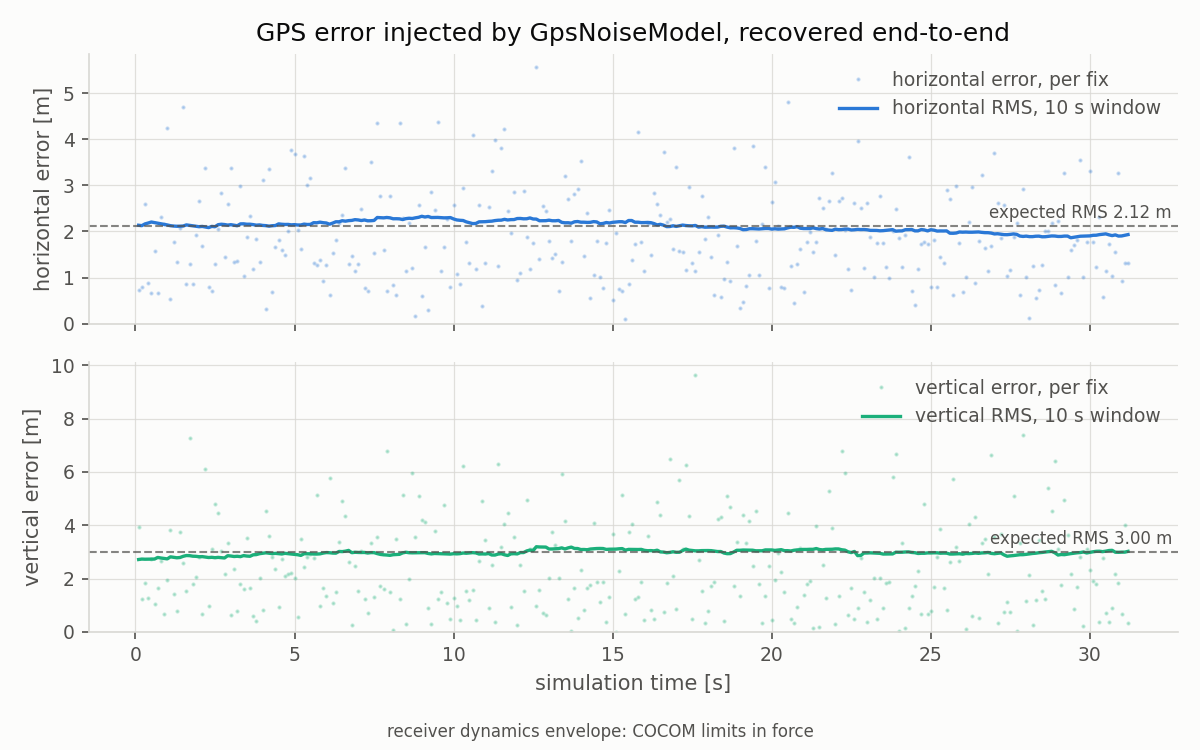
\includegraphics[width=\columnwidth]{gps_error.png}
\caption{Decoded-fix error against truth (faint points) with a 10\,s rolling RMS
(solid). Horizontal magnitude sits on the expected $1.5\sqrt{2}=2.12$\,m and
vertical on 3\,m: the chain adds nothing. The x-axis is the 31\,s a
COCOM-limited receiver leaves.}
\label{fig:gpserror}
\end{figure}

\subsection{The fix goes when both limits hold}
Fig.~\ref{fig:availability} and Fig.~\ref{fig:altitude} show the availability
consequence. The vehicle passes 515\,m/s at $t=10.1$\,s with nothing
happening---it is only 2\,km up---and loses the fix when it crosses 18\,km at
$t=31.2$\,s already doing 2\,km/s, both conditions then holding to the end. The
receiver reports 312 fixes out of 2001 epochs; the remaining 169\,s, including
all of stage 2, are unnavigated. Flight software that assumes GNSS through boost
is shown otherwise---and shown the useful version, the 31\,s of good data a
launch-detect or initialization routine actually gets.

\begin{figure}[t]
\centering

\includegraphics[width=\columnwidth]{gps_availability.png}
\caption{Altitude and speed against the COCOM thresholds; every no-fix epoch is
shaded. The AND sets the moment: 515\,m/s at $t=10.1$\,s does nothing, the fix
goes at 18\,km ($t=31.2$\,s).}
\label{fig:availability}
\end{figure}

\begin{figure}[t]
\centering

\includegraphics[width=\columnwidth]{altitude_vs_time.png}
\caption{Truth altitude with the decoded fixes over the first 31\,s; the
remaining 169\,s is the shaded outage, told in the data the flight software
actually received.}
\label{fig:altitude}
\end{figure}

\subsection{The byte chain is lossless}
The mission profile reads straight off the decoded IMU stream
(Fig.~\ref{fig:sf}), the cheapest sanity check on the plant there is:
${\sim}54$\,m/s$^2$ at lift-off rising to 125\,m/s$^2$ as stage 1 burns off,
\emph{exactly zero through the 94\,s coast} (an accelerometer does not sense
gravity), 57\,m/s$^2$ when stage 2 lights, 265\,m/s$^2$ at burnout, then zero.
Over the run, $20{,}000$ of $20{,}010$ inertial samples were decoded across
48{,}021 chip-select-framed SPI transfers with \emph{zero} checksum errors,
\emph{zero} FIFO overflows and \emph{zero} failed transfers; all 2001 NAV-PVT
frames were decoded (0 checksum errors); $2{,}000$ barometric conversions were
read and compensated across $42{,}009$ I$^2$C transactions with none failed; and
the magnetometer's 574 measurements crossed $2{,}368$ I$^2$C transactions, again
with none failed. The ten absent inertial samples are those the FMU buffered
before the flight computer probed and reset the FIFO---a driver clearing what
accumulated before it took over. The whole chain, from 6-DoF truth through four
noise models, four encoders, three transports and the on-target drivers, is
lossless and wire-correct. Fig.~\ref{fig:rates} shows the same fidelity in the
gyro channel, where the visible LSB banding is the quantization the flight
software must live with on the real part.

Sample \emph{counts} differ by two orders of magnitude between the SPI and
I$^2$C parts for a structural reason worth stating: the IMU FMU buffers ten
samples per communication step into a FIFO the controller drains in bursts,
while the two I$^2$C parts hold one conversion in unshadowed data registers and
a controller polling slower than the programmed rate simply observes the newest.
The magnetometer's 574 measurements over 200\,s are what a host-paced
co-simulation delivered against a 50\,Hz programmed rate, not a property of the
part. That is the honest reading of a polled-part sample count, and it is the
same reading a real slow consumer would get.

\begin{figure}[t]
\centering

\includegraphics[width=\columnwidth]{imu_specific_force.png}
\caption{Body-X specific force: truth vs.\ samples burst from the FIFO and
converted from raw counts. The full Scenario 17 profile is legible, including
zero through the coast. The receiver is COCOM-dark for 169 of these 200\,s,
including all of stage 2, and the inertial stream is indifferent to that---which
is the point of carrying an IMU.}
\label{fig:sf}
\end{figure}

\begin{figure}[t]
\centering

\includegraphics[width=\columnwidth]{imu_body_rates.png}
\caption{Body rates: the damped pitch oscillation during atmospheric flight,
tracked by decoded gyro samples. The horizontal banding is LSB quantization
(1 count $\approx 0.0011$\,rad/s at $\pm2000\,^\circ$/s) resolving the noise
floor.}
\label{fig:rates}
\end{figure}

\subsection{The barometer stops being an altimeter}
The BMP390 channel (Fig.~\ref{fig:baroalt}) is the complement to the GPS
result, and it fails for an unrelated reason. Compensated pressure decoded by
the on-target driver rides the ISA curve down from $101{,}321$\,Pa on the
pad---the sea-level value arrived at through the part's own compensation
arithmetic---and then flatlines near $10{,}450$\,Pa from $t\approx50$\,s, where
the reference part's ADC bottoms out. Inverted through the ISA, as flight
software does with a static-pressure measurement, the altimeter is honest to
$\sim$16\,km and then stops being an altimeter while the vehicle climbs another
220\,km.

The agreement below the range floor is the load-bearing part. The FMU produced
those raw words by \emph{inverting} the Bosch compensation polynomial and the
driver recovered pascals by running it \emph{forward}, with the coefficients
travelling across the bus as the 21 NVM bytes a physical part serves. A
value-level barometer FMU would have agreed with itself; this one agrees with an
independent execution of the manufacturer's published arithmetic, over a
register interface, and the range floor it inherits is the reference part's
rather than a modelling choice.

\begin{figure}[t]
\centering
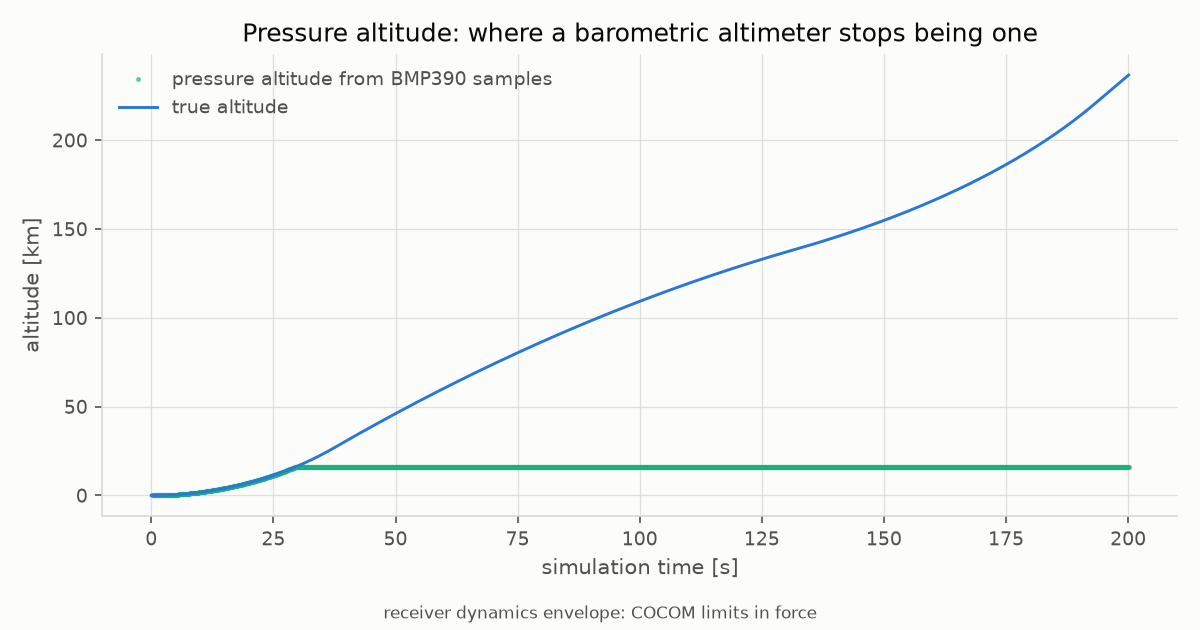
\includegraphics[width=\columnwidth]{baro_altitude.png}
\caption{Pressure altitude from decoded BMP390 samples against truth. The part
is an altimeter to $\sim$16\,km and then is not, while the vehicle climbs
another 220\,km---the barometric counterpart to the receiver's COCOM cut-off,
and the reason a launch vehicle carries several sensors at once.}
\label{fig:baroalt}
\end{figure}

\subsection{The magnetometer is unusable until it is conditioned}
\label{sec:magresults}
The magnetometer is where a register-accurate model earns its cost outright.
On the run reported here the simulated part was born with a bridge offset of
$+2656/{-}1690/{+}1395$~LSB, i.e.\ $+16.21/{-}10.31/{+}8.51$~\textmu T, against
a field of about 30~\textmu T. The on-target driver's SET/RESET pair measured
it at bring-up and removed it, and every sample afterwards is a field rather
than a field plus an unknown vector of its own size. Over the flight the
decoded field magnitude ran from 30.6 down to 27.2~\textmu T---the
$1/r^3$ falloff over 236\,km, plus the eastward translation of 2000\,km
relative to the dipole axis.

Fig.~\ref{fig:magfield} plots the three body axes rather than the magnitude,
deliberately. The axes are doing three different things---body $Y$ carries
almost the whole field because the vehicle flies due east across a
mostly-northward one, while $X$ and $Z$ hold the small residue as it pitches
over---which is exactly the geometry a swapped axis or a sign error destroys and
exactly what a magnitude plot hides. The constant gap between decoded samples
and the truth handed to the FMU is the simulated installation's hard iron,
present by design and not removed by conditioning.

Fig.~\ref{fig:magerror} quantifies what skipping the conditioning would have
cost, drawn from the same samples with the measured bridge offset added back:
$28$--$29^\circ$ of direction error on this run, and tens of degrees on any run,
since $\delta$ is redrawn each time from the datasheet's tolerance. The first
version of that figure plotted the uncalibrated \emph{magnitude}, and the two
curves nearly coincided---which is true, and is precisely why magnitude is the
wrong place to look: adding an offset the size of Earth's field to a field that
size barely changes the length of the vector while swinging its direction most
of a right angle. Heading is what a magnetometer is for, so the angle is the
honest measure of the damage. This is the paper's sharpest instance of the
central claim. Firmware that never runs the SET/RESET sequence produces a
plausible-looking field stream, passes every value-level check, and is wrong by
roughly $100\%$; no idealized sensor FMU can present that failure, because there
is no bridge in a floating-point number.

\begin{figure}[t]
\centering
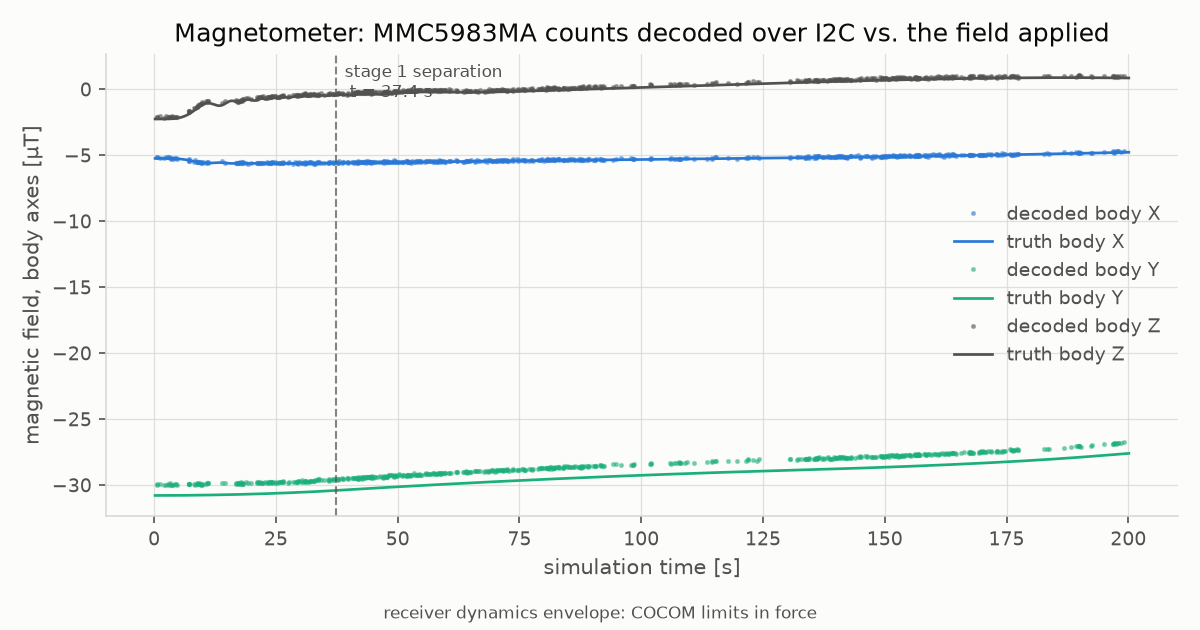
\includegraphics[width=\columnwidth]{mag_body_field.png}
\caption{Body-frame field decoded by the on-target \code{Mmc5983maDriver} over
the simulated I$^2$C bus, against the truth field the FMU was handed. Plotted
per axis, because the axis geometry is what a sign or ordering error destroys.
The constant offset is the simulated installation's hard iron, which SET/RESET
does not remove and is not meant to.}
\label{fig:magfield}
\end{figure}

\begin{figure}[t]
\centering
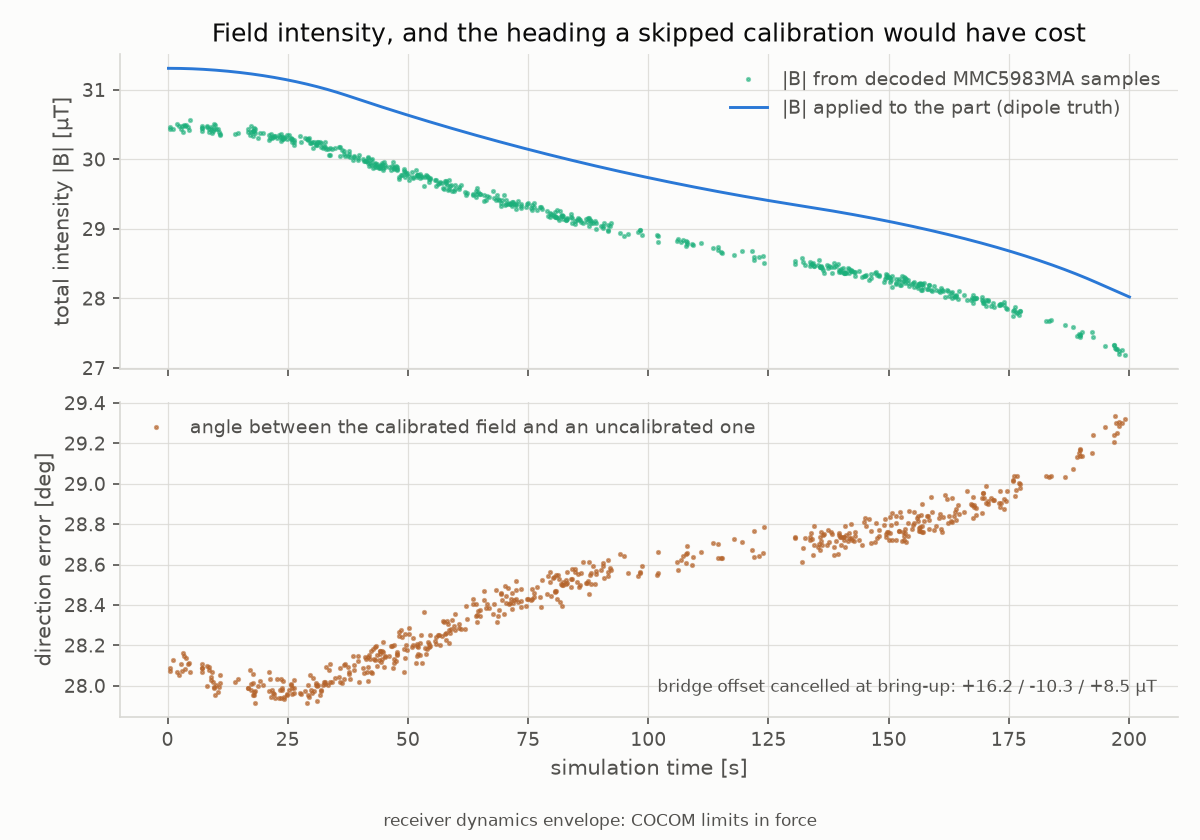
\includegraphics[width=\columnwidth]{mag_magnitude.png}
\caption{Top: total intensity over the flight, 30.6 down to
27.2\,\textmu T. Bottom: the direction error a skipped SET/RESET calibration
would have caused, reconstructed by adding the measured bridge offset back into
the same samples---$28$--$29^\circ$ on this run. Magnitude barely moves while
heading swings most of a right angle, which is why the angle is the honest
measure.}
\label{fig:magerror}
\end{figure}

\subsection{One honest artifact}
Unpaced, the co-simulation is not uniformly fast---in-atmosphere powered flight
costs real time (DAVE-ML table lookups on every implicit Radau stage) while
coasting is cheap---so where the master accelerates it can outrun the poll loop
and overflow the FIFO, losing a few hundred of 20{,}010 samples. The sticky
overflow bit reports it and no frame is ever truncated: this is exactly what a
FIFO plus overflow flag exists to give. It is an artifact of the simulation, not
of the system under test---a real plant cannot outrun its consumer---and pacing
the master to wall-clock removes it. That the harness \emph{surfaces} the
condition rather than hiding it is itself a property worth having.

% ===========================================================================
\section{Discussion}
% ===========================================================================
\textbf{Same code across three tiers.} The decoders validated above are the
identical translation units that run inside Renode's instruction-accurate STM32
simulation and on physical STM32H743 hardware; only the bus shim beneath the
driver changes (UDP or shared memory here, \code{HAL\_SPI\_TransmitReceive} or
\code{HAL\_I2C\_Mem\_Read} plus GPIO on the target). For the barometer this is
measured rather than asserted: a software-in-the-loop test gates in continuous
integration that runs the cross-compiled H743 firmware inside Renode, through
Renode's emulated I$^2$C controller, a C\# bridge peripheral, a TCP hop and the
shared-memory bus, against the same \code{Bmp390I2cSlave} the FMU embeds. The
equivalent magnetometer loop is written and registered but has not yet executed
end to end; every layer beneath it is separately verified, including the full
blocking SET/RESET handshake across the real shared-memory transport, and the
unexercised span is only the Renode/C\#/TCP legs the barometer loop already
covers. Its load-bearing assertion is not the field values but that the bridge
offset the firmware reports matches the one the peripheral independently reports
having been born with---the one comparison that separates conditioned firmware
from firmware that merely prints plausible numbers. SIL results therefore
transfer to HIL with a validity a value-level harness cannot claim, because the
code that most often breaks on hardware is the code SIL usually omits.

\textbf{Conformance as a side effect.} Because neither sensor FMU hand-writes
the FMI export table---a \code{fmu4cpp}~\cite{fmu4cpp} layer exports the full
table and the model description is \emph{generated} from the registered
variables---the description and binary cannot drift, and the archive passes a
strict loader (fmi4c resolves the complete 2.0 table up front and refuses a
binary that omits any function, even those whose capability flags are false).
Generating the description from the model is good conformance pressure any strict
master would exert.

\textbf{Limitations.} The error models are per-axis Gaussian with a turn-on bias
and quantization; they omit correlated in-run bias walk (Gauss-Markov), scale-
factor and misalignment errors, temperature dependence, and---for the
magnetometer---soft-iron distortion, which is deliberately excluded to keep the
diagonal inverse exactly equal to \code{convert\_raw\_to\_si()}. (Hard iron
\emph{is} modelled, as Section~\ref{sec:partmodels} describes, because it is a
field rather than a distortion and needs no inverse.) The magnetic environment
is a centred tilted dipole rather than a full spherical-harmonic model, which is
adequate for exercising a driver and inadequate for magnetic navigation,
particularly at the scenario's equatorial pad. The MMC5983MA's self-test coil is
modelled at the register level but not magnetically, so a driver self-test would
pass vacuously against the FMU; the shared-memory I$^2$C bus carries one
peripheral per bus, so multi-drop addressing is not exercised
(Section~\ref{sec:i2c}). The barometer carries a local ISA atmosphere as a
placeholder pending an environment model. The radar altimeter is the one sensor
of the five with a model but no case-study validation: the scenario is a launch
to orbit, and there is no ground under it to measure. The specific-force and magnetic-field
inputs and the master's between-step connection propagation each introduce one
communication step of transport delay, which the analysis accounts for but which
bounds timing fidelity to the communication rate. None of these affect the
paper's claim, which is about the \emph{transport and protocol} fidelity of the
sensor boundary, not the richness of the stochastic model behind it; richer
error models drop into~\eqref{eq:errormodel} without changing the pattern.

% ===========================================================================
\section{Conclusion}
% ===========================================================================
Value-level sensor FMUs let SIL co-simulation test everything about GNC software
except the byte-level driver and protocol code that fails most on real hardware.
We showed that this shortcut is avoidable: protocol-accurate sensor FMUs take
truth in over FMI and answer the part's real bus---wire-exact frames where the
part frames, register bursts where it does not---with no FMI outputs, so the
unmodified flight-software decoder is exercised against exactly what it will see
in flight. The pattern captures a talker/polled distinction across three
transports and in-flight behaviors a value-level model cannot express: a
receiver revoking its fix to export limits, a FIFO overflowing under a slow
consumer, a compensation polynomial that must be inverted before a barometer's
counts mean anything, and a magnetometer with no useful output at all until a
blocking multi-transaction handshake has separated its bridge offset from the
field. Its inverse-model property makes simulator and flight code mutually
self-checking. End-to-end against a verified two-stage-rocket plant, four
sensors decode losslessly across three transports, the decoded error equals the
injected error to quantization, and the conditioning sequence recovers a bridge
offset without which heading would be $28^\circ$ out. Future work extends the
stochastic models with correlated bias dynamics and the deferred soft-iron term,
closes the guidance loop with an onboard convex solver, and quantifies
SIL-to-HIL transfer on physical STM32 hardware.

% ===========================================================================
\section*{Reproducibility}
The framework, the seven sensor FMUs (five sensors, two of them at both
fidelity tiers), the case study, the Renode software-in-the-loop harnesses and
the plotting scripts are open source under GPLv3. Each sensor FMU is exported
for both FMI 2.0 and 3.0 from one source, and every model constructor accepts an
RNG seed---so a run's turn-on biases, hard iron and bridge offset are
reproducible bit for bit, which is what makes a figure like
Fig.~\ref{fig:magerror} checkable rather than merely illustrative.

\section*{Acknowledgment}
% Fill in funding / institutional acknowledgments before submission.

\bibliographystyle{IEEEtran}
\bibliography{references}

\end{document}
